%% Beginning of file 'SN2020jgb.tex'
%% using aastex version 6.3
\documentclass[twocolumn]{aastex631}

\newcommand\sn{SN\,2020jgb}
\newcommand\trpeak{$t_{r,\mathrm{peak}}$}
\newcommand\tfl{$t_\mathrm{fl}$}

\shorttitle{\sn}
\shortauthors{Authors et al.}
\graphicspath{{./}{figures/}}

\begin{document}

\title{\sn}

\author{Authors}
\affiliation{Center for Interdisciplinary Exploration and Research in Astrophysics (CIERA), Department of Physics and Astronomy, Northwestern University, 2145 Sheridan Road, Evanston, IL 60208, USA}

\begin{abstract}

\end{abstract}

\keywords{keywords}

\section{Introduction} \label{sec:intro}
\section{Observations} \label{sec:obs}
\subsection{Detection and Classification}
\sn\ was first discovered by the Zwicky Transient Facility \citep[ZTF;][]{ZTF2019a,ZTF2019b} on 2020 May 03.463 UT (MJD 58972.463) with the 48-inch Samuel Oschin Telescope (P48) at Palomar Observatory. The internal designation is ZTF20aayhacx. It was detected at a magnitude of 19.86 in ZTF $g$-band, and J2000 coordinates $\alpha=17^\mathrm{h}53^\mathrm{m}12^\mathrm{s}.651$, $\delta=-00^\circ51'21''.81$. The last non-detection was on 2020 April 27.477 (MJD 58966.477; 5.99 days before the first detection) up to a limiting magnitude of 20.7 in ZTF $r$-band.

\textbf{Classification, ...}

\subsection{Optical Photometry}
We obtained $gr$-band photometry of \sn\ with the ZTF camera. A Galactic extinction of $E(B-V)=0.404$ is reported by the maps of \citet{Schlafly2011}, for which we correct all our photometry using the extinction model proposed by \citet{Fitzpatrick1999}. We do not account for any additional host extinction due to the lack of any \ion{Na}{1} D absorption in our spectra (\textbf{Is it in the outskirt?}).
\begin{figure*}
    \centering
    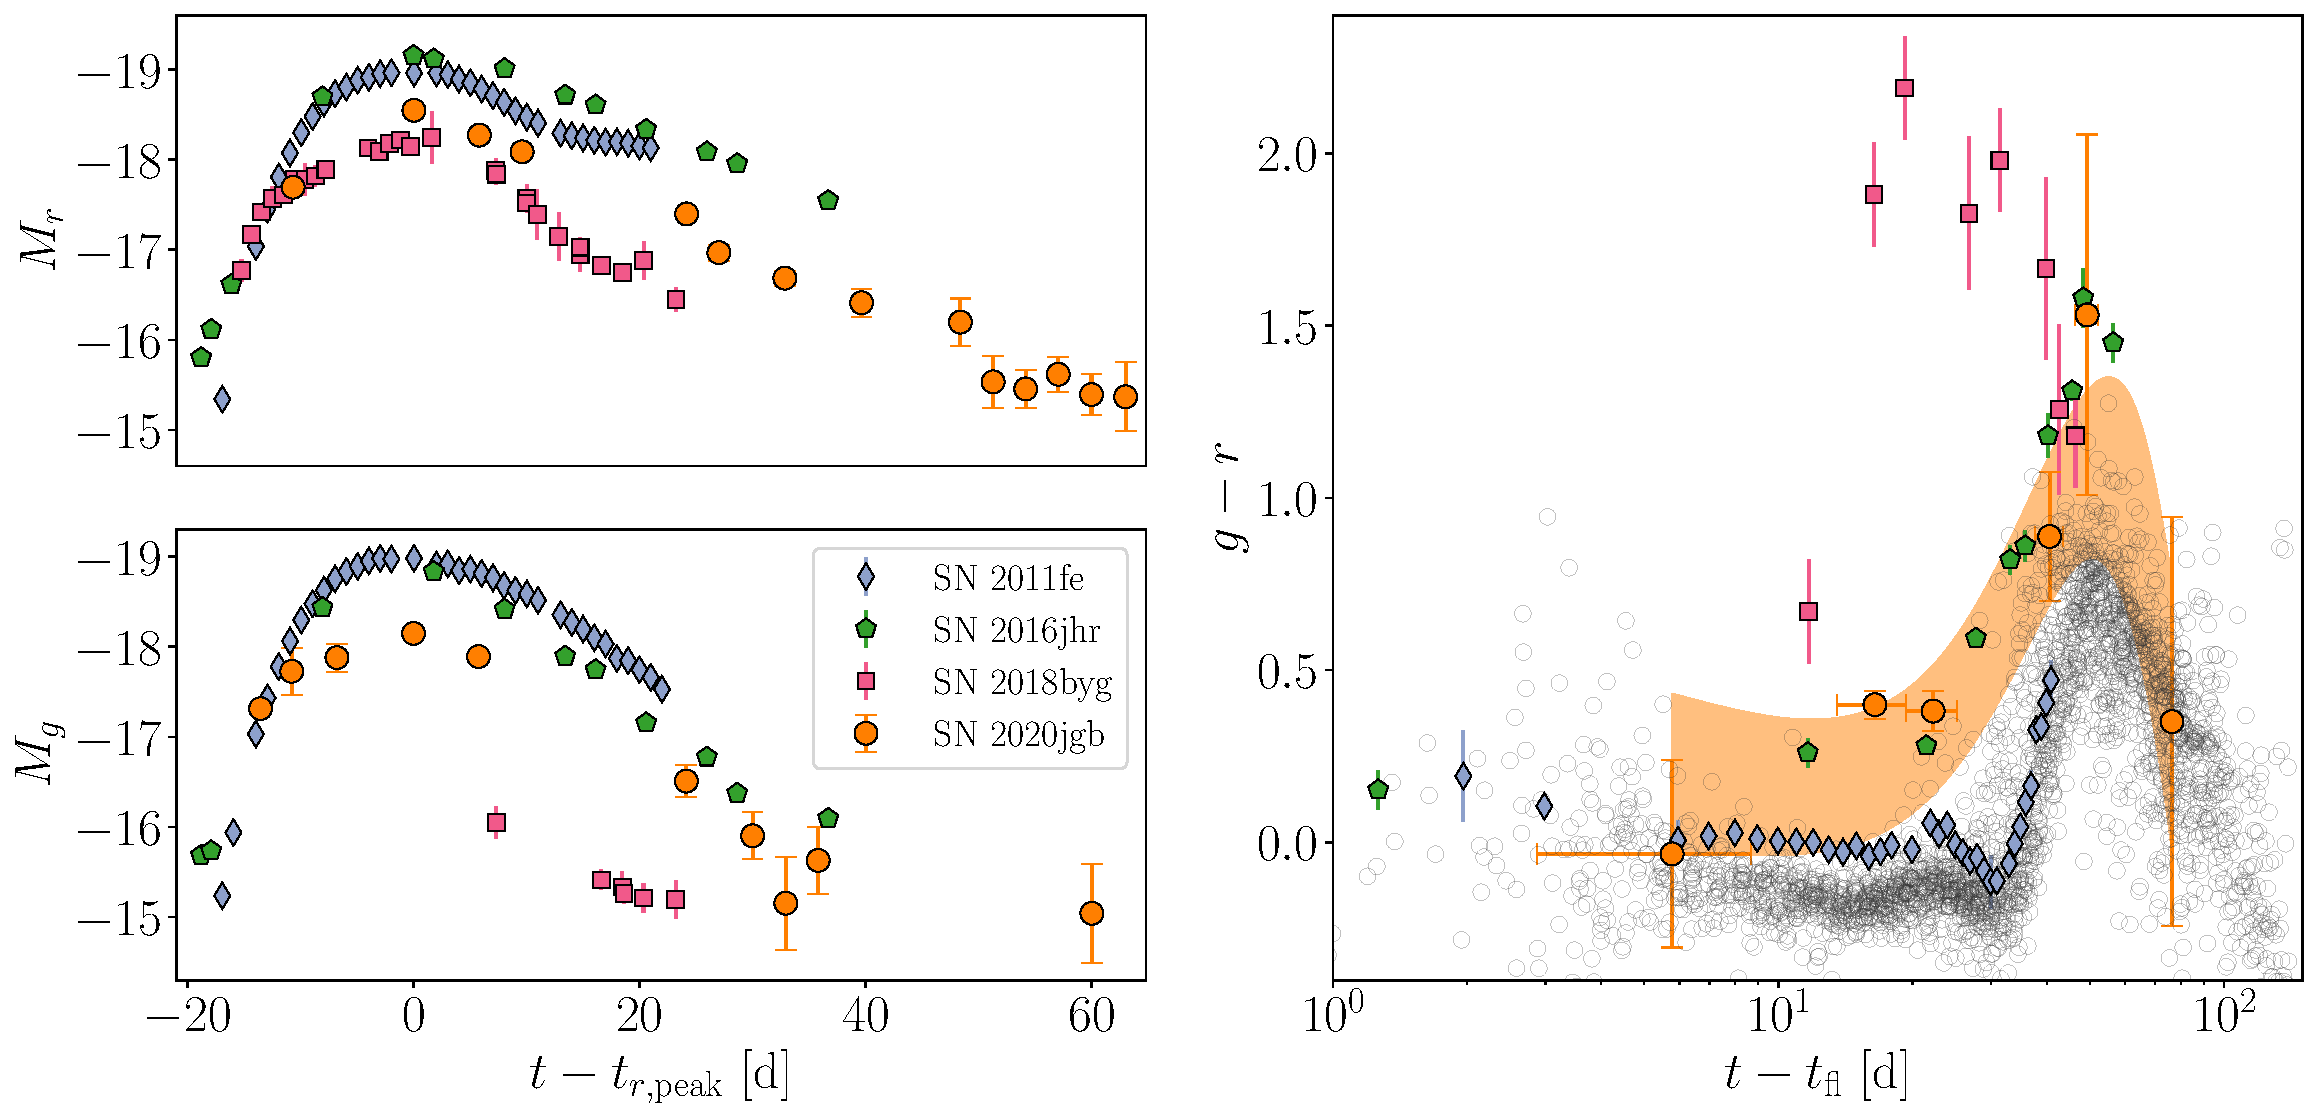
\includegraphics[width=\textwidth]{photometry.pdf}
    \label{fig:photometry}
    \caption{\textit{Left}: comparison of the multi-color ($g$ and $r$ bands) light curves of \sn\ to the normal SN Ia SN 2011fe and the He double detonation candidate SN 2018byg. \textit{Right}: comparison of $g-r$ color evolution to SN 2011fe and SN 2018byg, as well as 62 normal SNe Ia (open circles) with prompt observations within 5 days of first light by ZTF \citep{Bulla2020}. The shaded region denotes the 1-$\sigma$ credible interval of the color of SN 2020jgb until $\approx$40 days after the peak, estimated using Gaussian process.}
\end{figure*}

\subsection{Optical Spectroscopy}
\begin{deluxetable}{lrcccc}
\tabletypesize{\scriptsize}
\tablewidth{0pt}
\tablecaption{Spectroscopic Observations of \sn\label{tab:spectra}}
\tablehead{
\colhead{$t_\mathrm{obs}$} &
\colhead{Phase} &
\colhead{Telescope/} &
\colhead{$R$} &
\colhead{Range} &
\colhead{Air} \\
\colhead{(MJD)} &
\colhead{(d)} &
\colhead{Instrument} &
\colhead{$(\lambda/\Delta\lambda)$} &
\colhead{(\AA)} & 
\colhead{Mass}
}
\startdata
58,976.42 &  $-$9.7 & P60/SEDM & 100 & 3770--9220 & 1.23\\
58,982.12 & $-$4.2 & NOT/ALFOSC & 360 & 4000--9620 & 1.17\\
58,990.43 &  $+$3.9 & P60/SEDM & 100 & 3770--9220 &  1.23\\
58,997.44 & $+$10.7 & P60/SEDM & 100 & 3770--9220 &  1.29\\
58,998.41 & $+$11.6 & Shane/Kast & 1000? & 3620--10720 & 1.28\\
59,008.41 & $+$21.3 & P60/SEDM & 100 & 3770--9220 & 1.28\\
59,010.40 & $+$23.3 & P200/DBSP & 700 & 3200--9500 &  1.27\\
59,023.58 & $+$36.1 & Keck I/LRIS & 1100 & 3200--10250 & 2.04\\
59,107.29 & $+$117.3 & Keck I/LRIS & 1100 & 3200--10250 & 1.31\\
59,143.26 & $+$152.2 & Keck I/LRIS & 1100 & 3200--10250 & 2.16\\
\enddata
\tablecomments{Phase is measured relative to \trpeak\ in the host galaxy rest frame. The resolution $R$ is reported for the central region of the spectrum.}
\end{deluxetable}
\begin{figure}
    \centering
    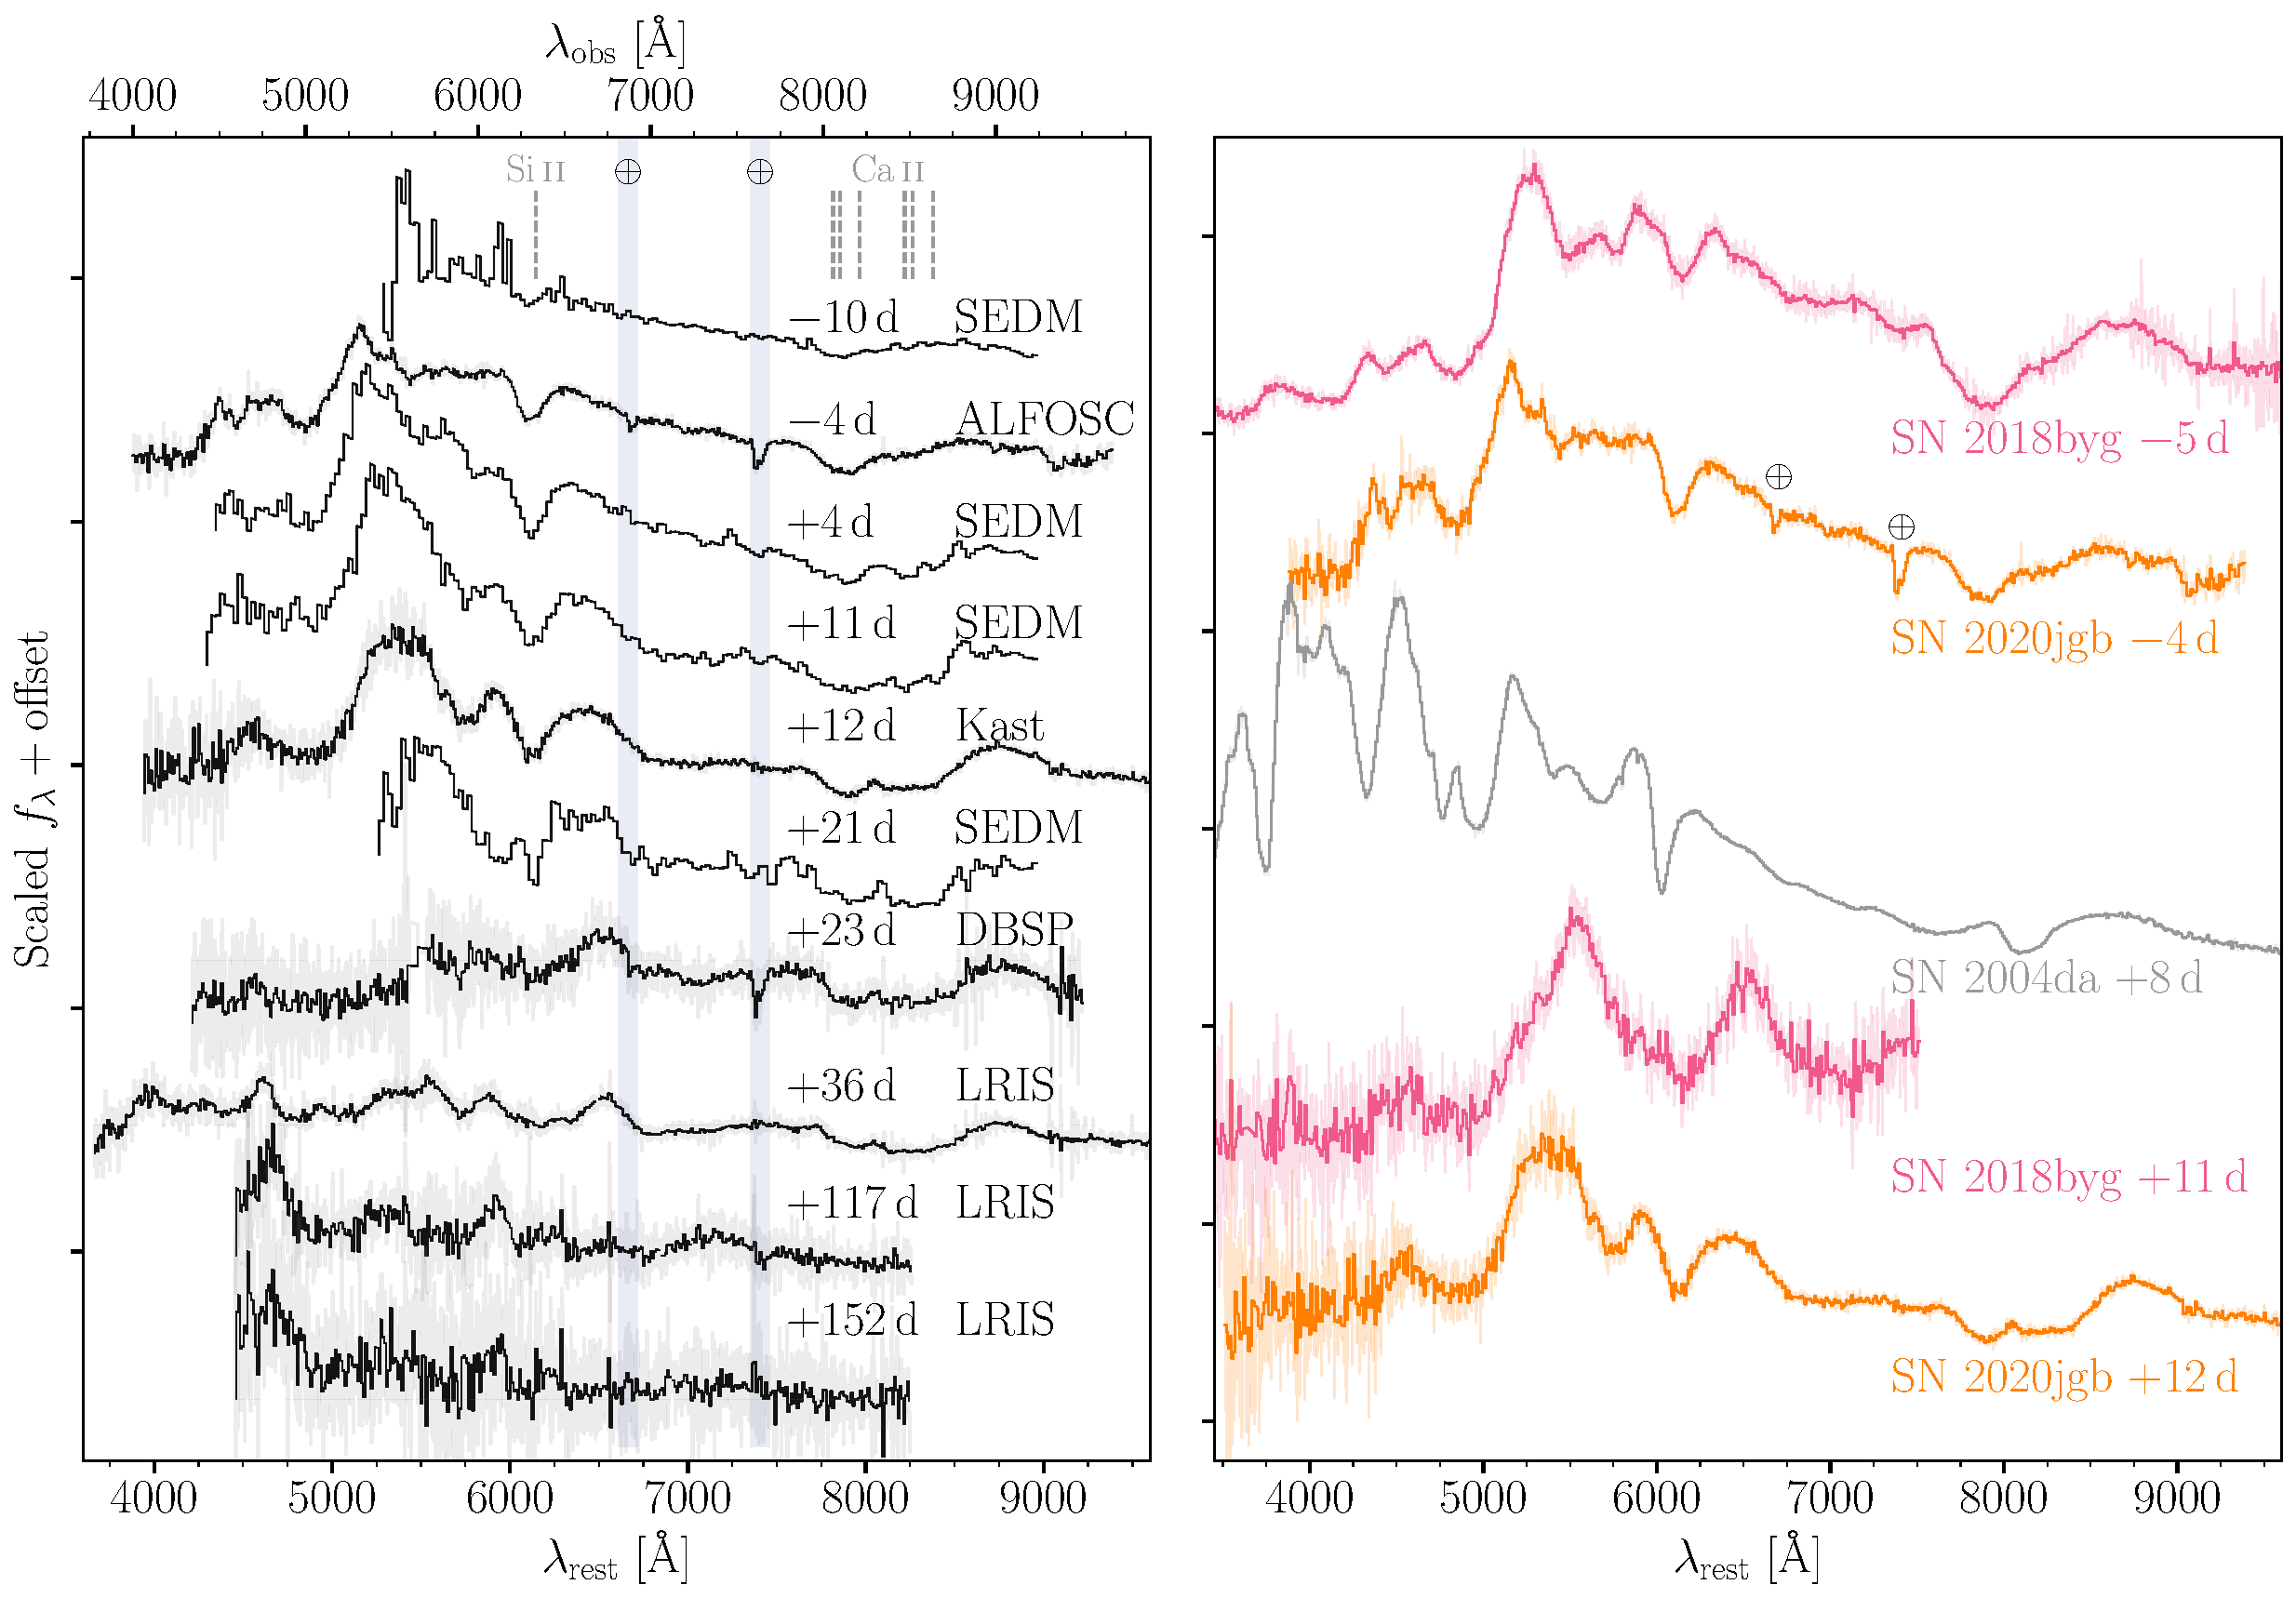
\includegraphics[width=\linewidth]{optical_spec_evolution.pdf}
    \caption{Optical spectroscopic sequence of \sn. Rest frame phases (days) relative to the $r$-band peak and instruments used are posted next to each spectrum. The black curves are binned spectra with a bin size of 10 \r{A}, except for the SEDm spectra, whose resolution is lower. The 1-$\sigma$ uncertainties of raw spectra are shown in grey. Only regions with SNR $>3$ after binning are plotted.} %The \ion{Si}{2} and \ion{Ca}{2} IRT absorption lines are indicated by the vertical dashed lines. The telluric lines are denoted by the earth symbol, ``$\earth$''.
    \label{fig:spec_evo}
\end{figure}

\subsection{Near-infrared (NIR) Spectroscopy}
We obtained one NIR spectrum of the transient using the Gemini near-infrared spectrometer \citep[GNIRS;][]{GNIRS1998} on the Gemini North telescope on 2020 June 9 ($\approx$22 days after $r$-band peak), for an integration time of 2400 s. The spectra were reduced with the \texttt{PypeIt} Python package \citep{pypeit:joss_pub,pypeit:zenodo}.

\section{Analysis} \label{sec:analysis}
\subsection{Photometric Properties}
\begin{itemize}
    \item sub-luminous
    \item first light time, peak time
    \item color evolution
\end{itemize}

\subsection{Spectroscopic Properties}
\begin{itemize}
    \item infrared \ion{Ca}{2} triplet (\ion{Ca}{2} IRT)
    \item tentative \ion{He}{1} absorption at $\approx$1 \micron
\end{itemize}
\subsection{NIR spectra}
In Figure~\ref{fig:NIR_spec}, the NIR spectrum is presented along with three spectra in the sample of \cite{Marion2009_NIR} at similar phases. \sn\ shows a strong absorption feature at $\approx$0.99 \micron, which is not seen in normal SNe Ia. This feature was still prominent two weeks later, as detected by LRIS on Keck (see Figure~\ref{fig:hvf_comp}), though it was only partially covered due to the limitation of bandwidth. In general, \sn\ highly resembles normal SNe Ia in NIR band. The shape of the continuum redwards to $\approx$1.2 \micron\ is significantly altered by line-blanketing of Fe-group elements synthesized in the SN interior, as opposed to the Fe-group elements in the outermost region as ashes of shell helium burning. Just like normal SNe Ia, \sn\ also show enhancement of flux at about 1.3, 1.55, 2.0, 2.1, and 2.25 \micron, accompanied by several \ion{Co}{2} absorption lines. It is especially similar to SN 2004da at +25 days after maximum as the increase in flux at $\approx$1.55 \micron, known as the \textit H-band break, has become less prominent. %For many other SNe Ia, however, the \textit H-band break can last till much later stages \citep{Marion2009_NIR}.
\begin{figure*}
    \centering
    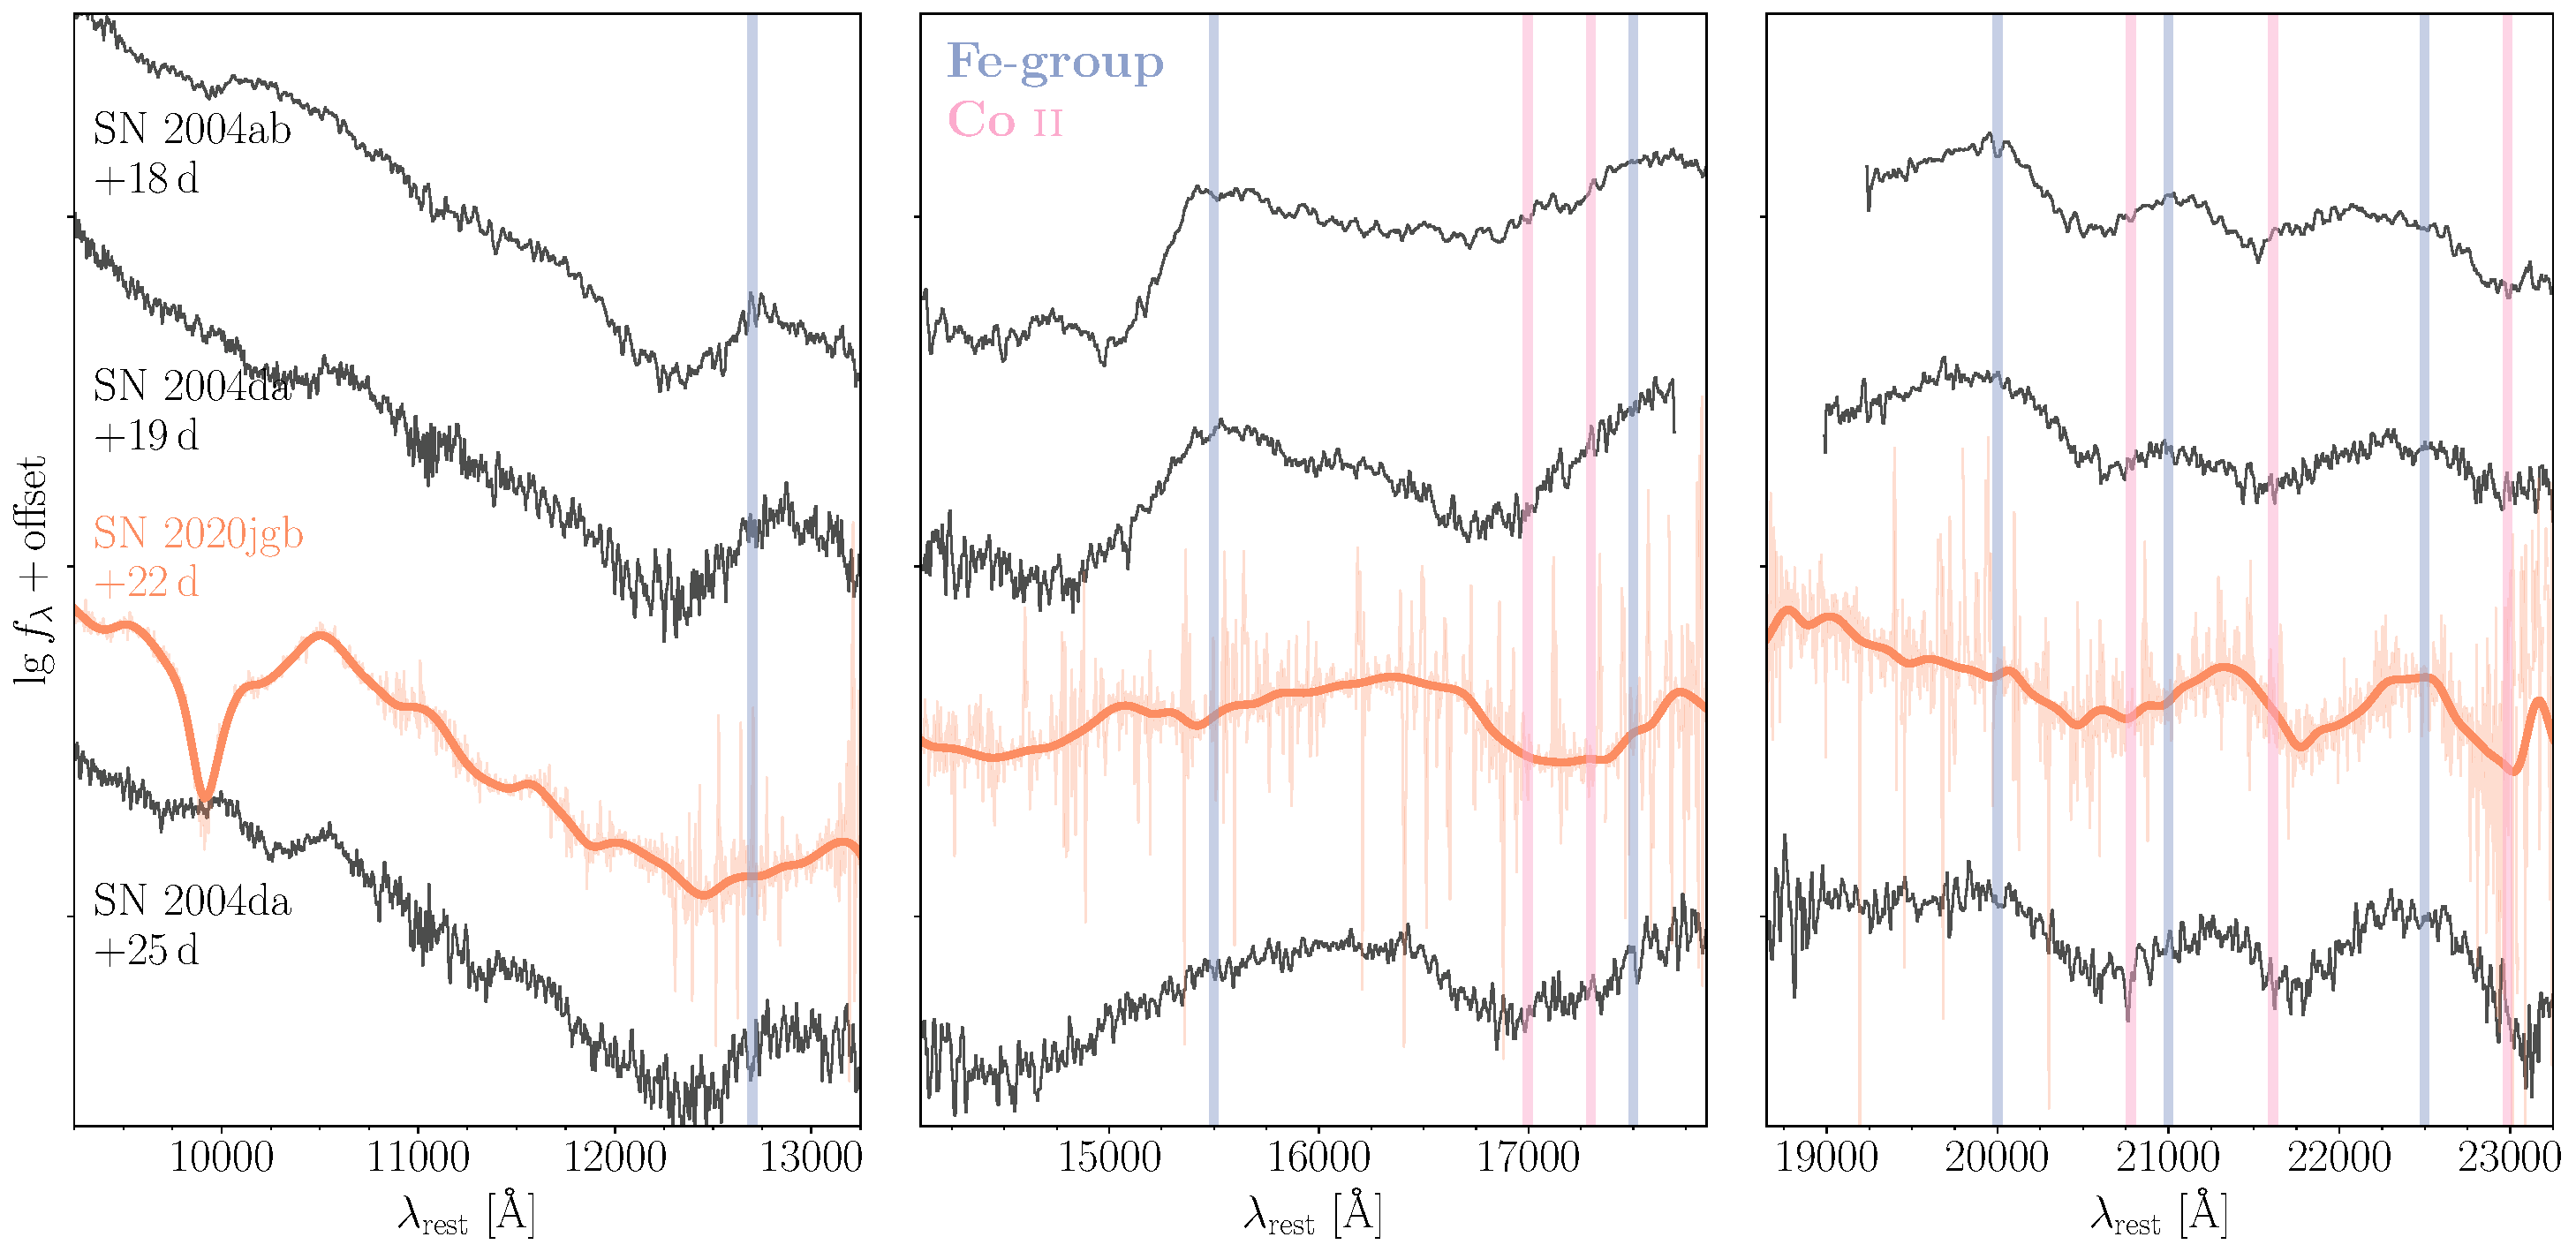
\includegraphics[width=\textwidth]{NIR_spec.pdf}
    \caption{The NIR spectra of \sn\ and two SNe Ia with normal maximum luminosity \citep[SN 2004ab and SN 2004da,][]{Marion2009_NIR}, taken about three weeks after the peak. For each spectrum, the continuum at $\gtrsim1.2$ \micron\  is significantly reshaped by the Fe-group blanketing (emission features, blue vertical lines) and \ion{Co}{2} absorption (pink vertical lines).}
    \label{fig:NIR_spec}
\end{figure*}

What is not seen in usual SNe Ia is the wide, deep absorption at $\approx$0.99 \micron, indicating its peculiarity. According to \citet{Marion2009_NIR}, normal SNe Ia are nearly featureless in spectra around 1 \micron\ a few weeks past the week. After $\sim$3 weeks, some \ion{Fe}{2} features (0.9998 \& 1.0500 \micron) start to develop, but are not even nearly as prominent as the 0.99 \micron\ feature. However, there are other He-shell double detonation candidates showing complexity in this region. In the currently small sample of five candidates, two objects (SN 2016jhr and SN 2019ofm) do not have any available NIR spectra, while the other three all exhibit strong absorption features near 1 \micron, though the spectra were obtained at different phases, as shown in Figure~\ref{fig:NIR_comp}. The 1 \micron\ feature for SN 2016hnk lies slightly redder than the other two, which corresponds to an expansion velocity lower by $\sim$3,000 km/s, assuming they all have the same origin. 

\begin{figure}
    \centering
    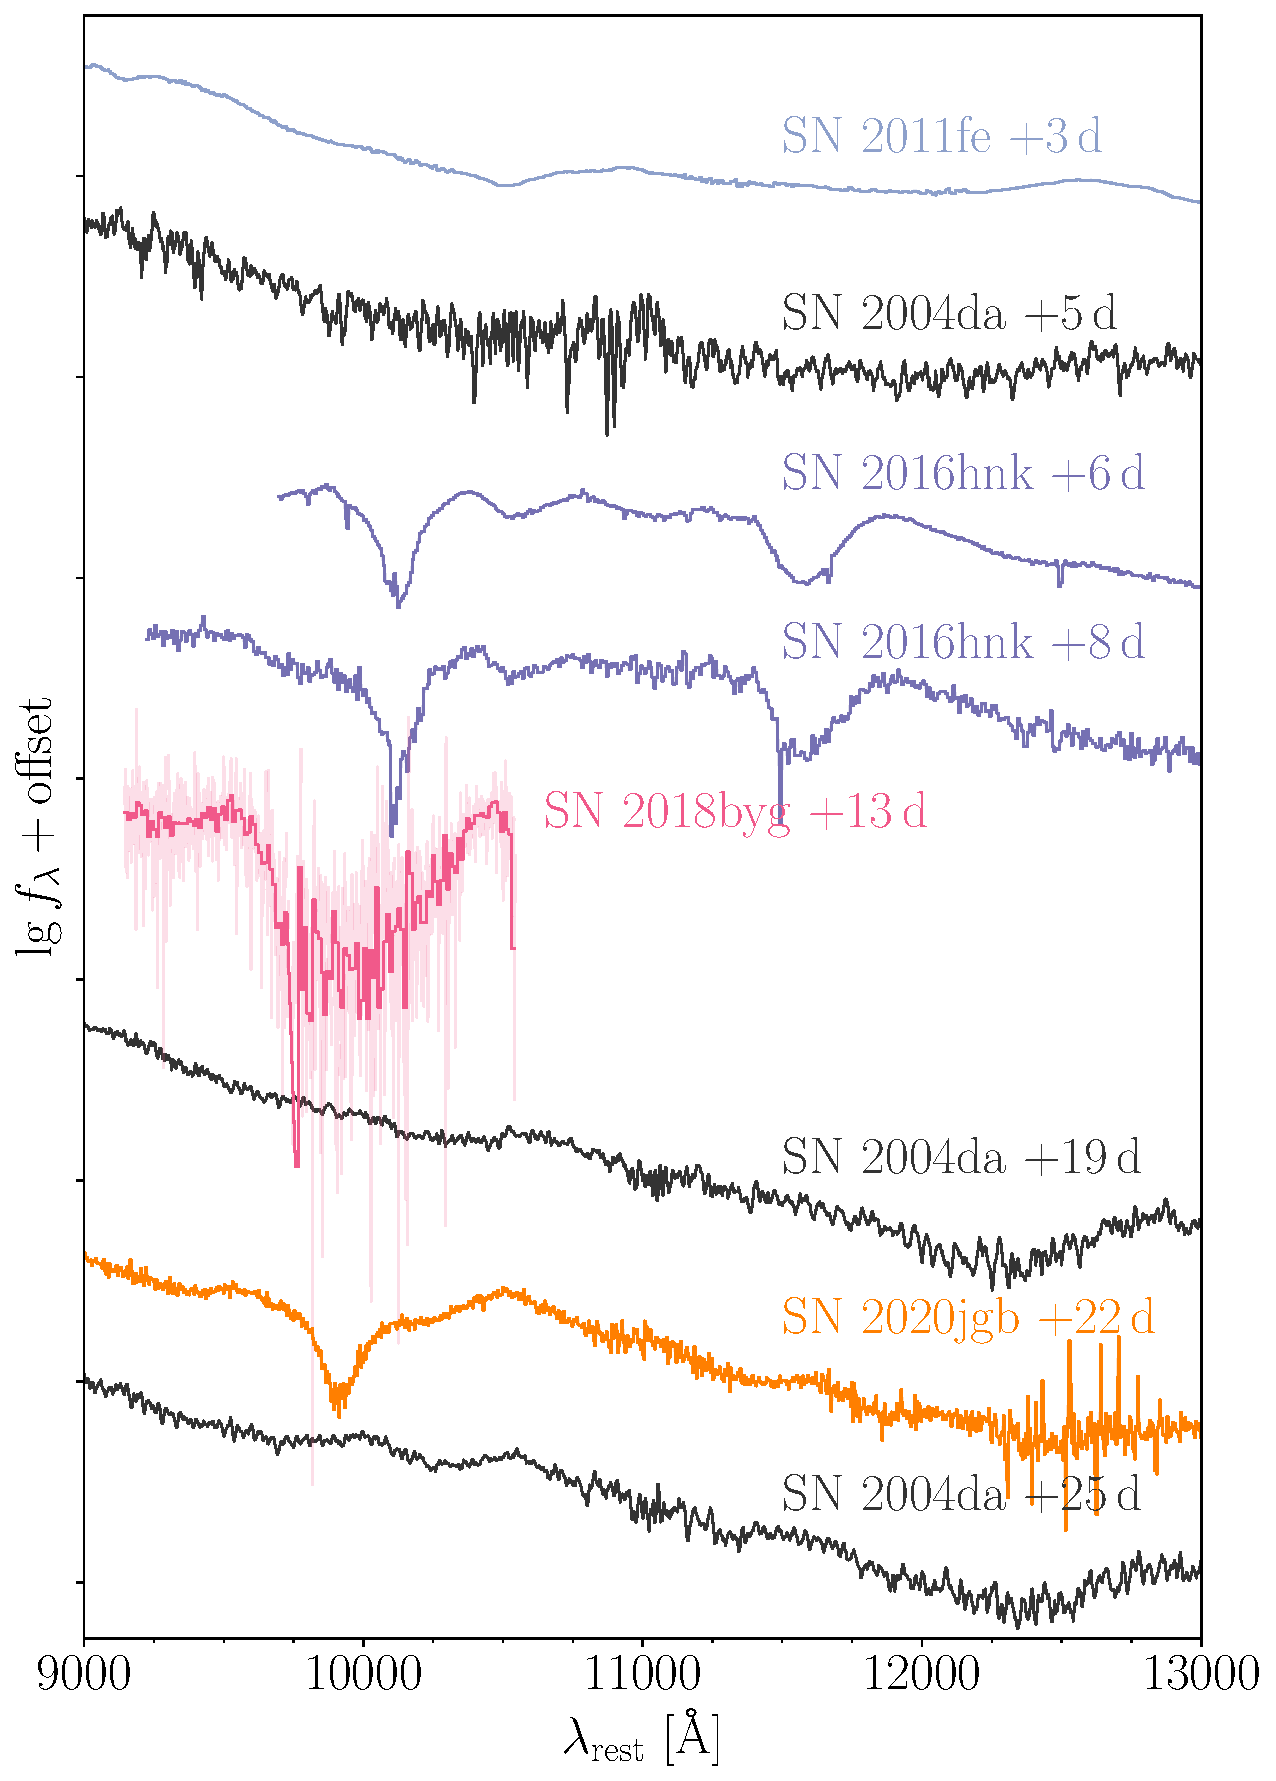
\includegraphics[width=\linewidth]{NIR_spec_comp.pdf}
    \caption{The NIR spectra (9,000 to 13,000 \AA) of a few normal SNe Ia (SN 2011fe and SN 2004da) and three He-shell double detonation candidates, which are all subluminous SNe Ia (SN 2016hnk, SN 2018byg, and this source, \sn).}
    \label{fig:NIR_comp}
\end{figure}

There are several elements that may be associated with this feature, none of which is fully satisfying. The most attractive possibility is the strong \ion{He}{1} line at 1.0830 \micron, as has predicted in sub-Chandrasekhar-mass He-shell double detonation models when considerable amount of helium in the shell is left unburnt \citep{Boyle2017_Helium}. Figure~\ref{fig:hvf_comp} shows that the 1 \micron\ feature, if associated with \ion{He}{1} $\lambda$1.0830 \micron, has a high velocity ($\approx$26,000 km/s), yet similar as the HVF of \ion{Ca}{2} IRT ($\approx$24,000 km/s). The expansion velocity in the ejecta is roughly linearly proportional to the radius, so such a high velocity indicates that both the \ion{Ca}{2} IRT and the tentative \ion{He}{1} absorption line form far outside the normal photosphere, which has a velocity of only $\approx$10,000 km/s. In the sense, the He-shell double detonation scenario, in which the unburnt helium locates at the outermost ejecta, is indeed supported.
\begin{figure}
    \centering
    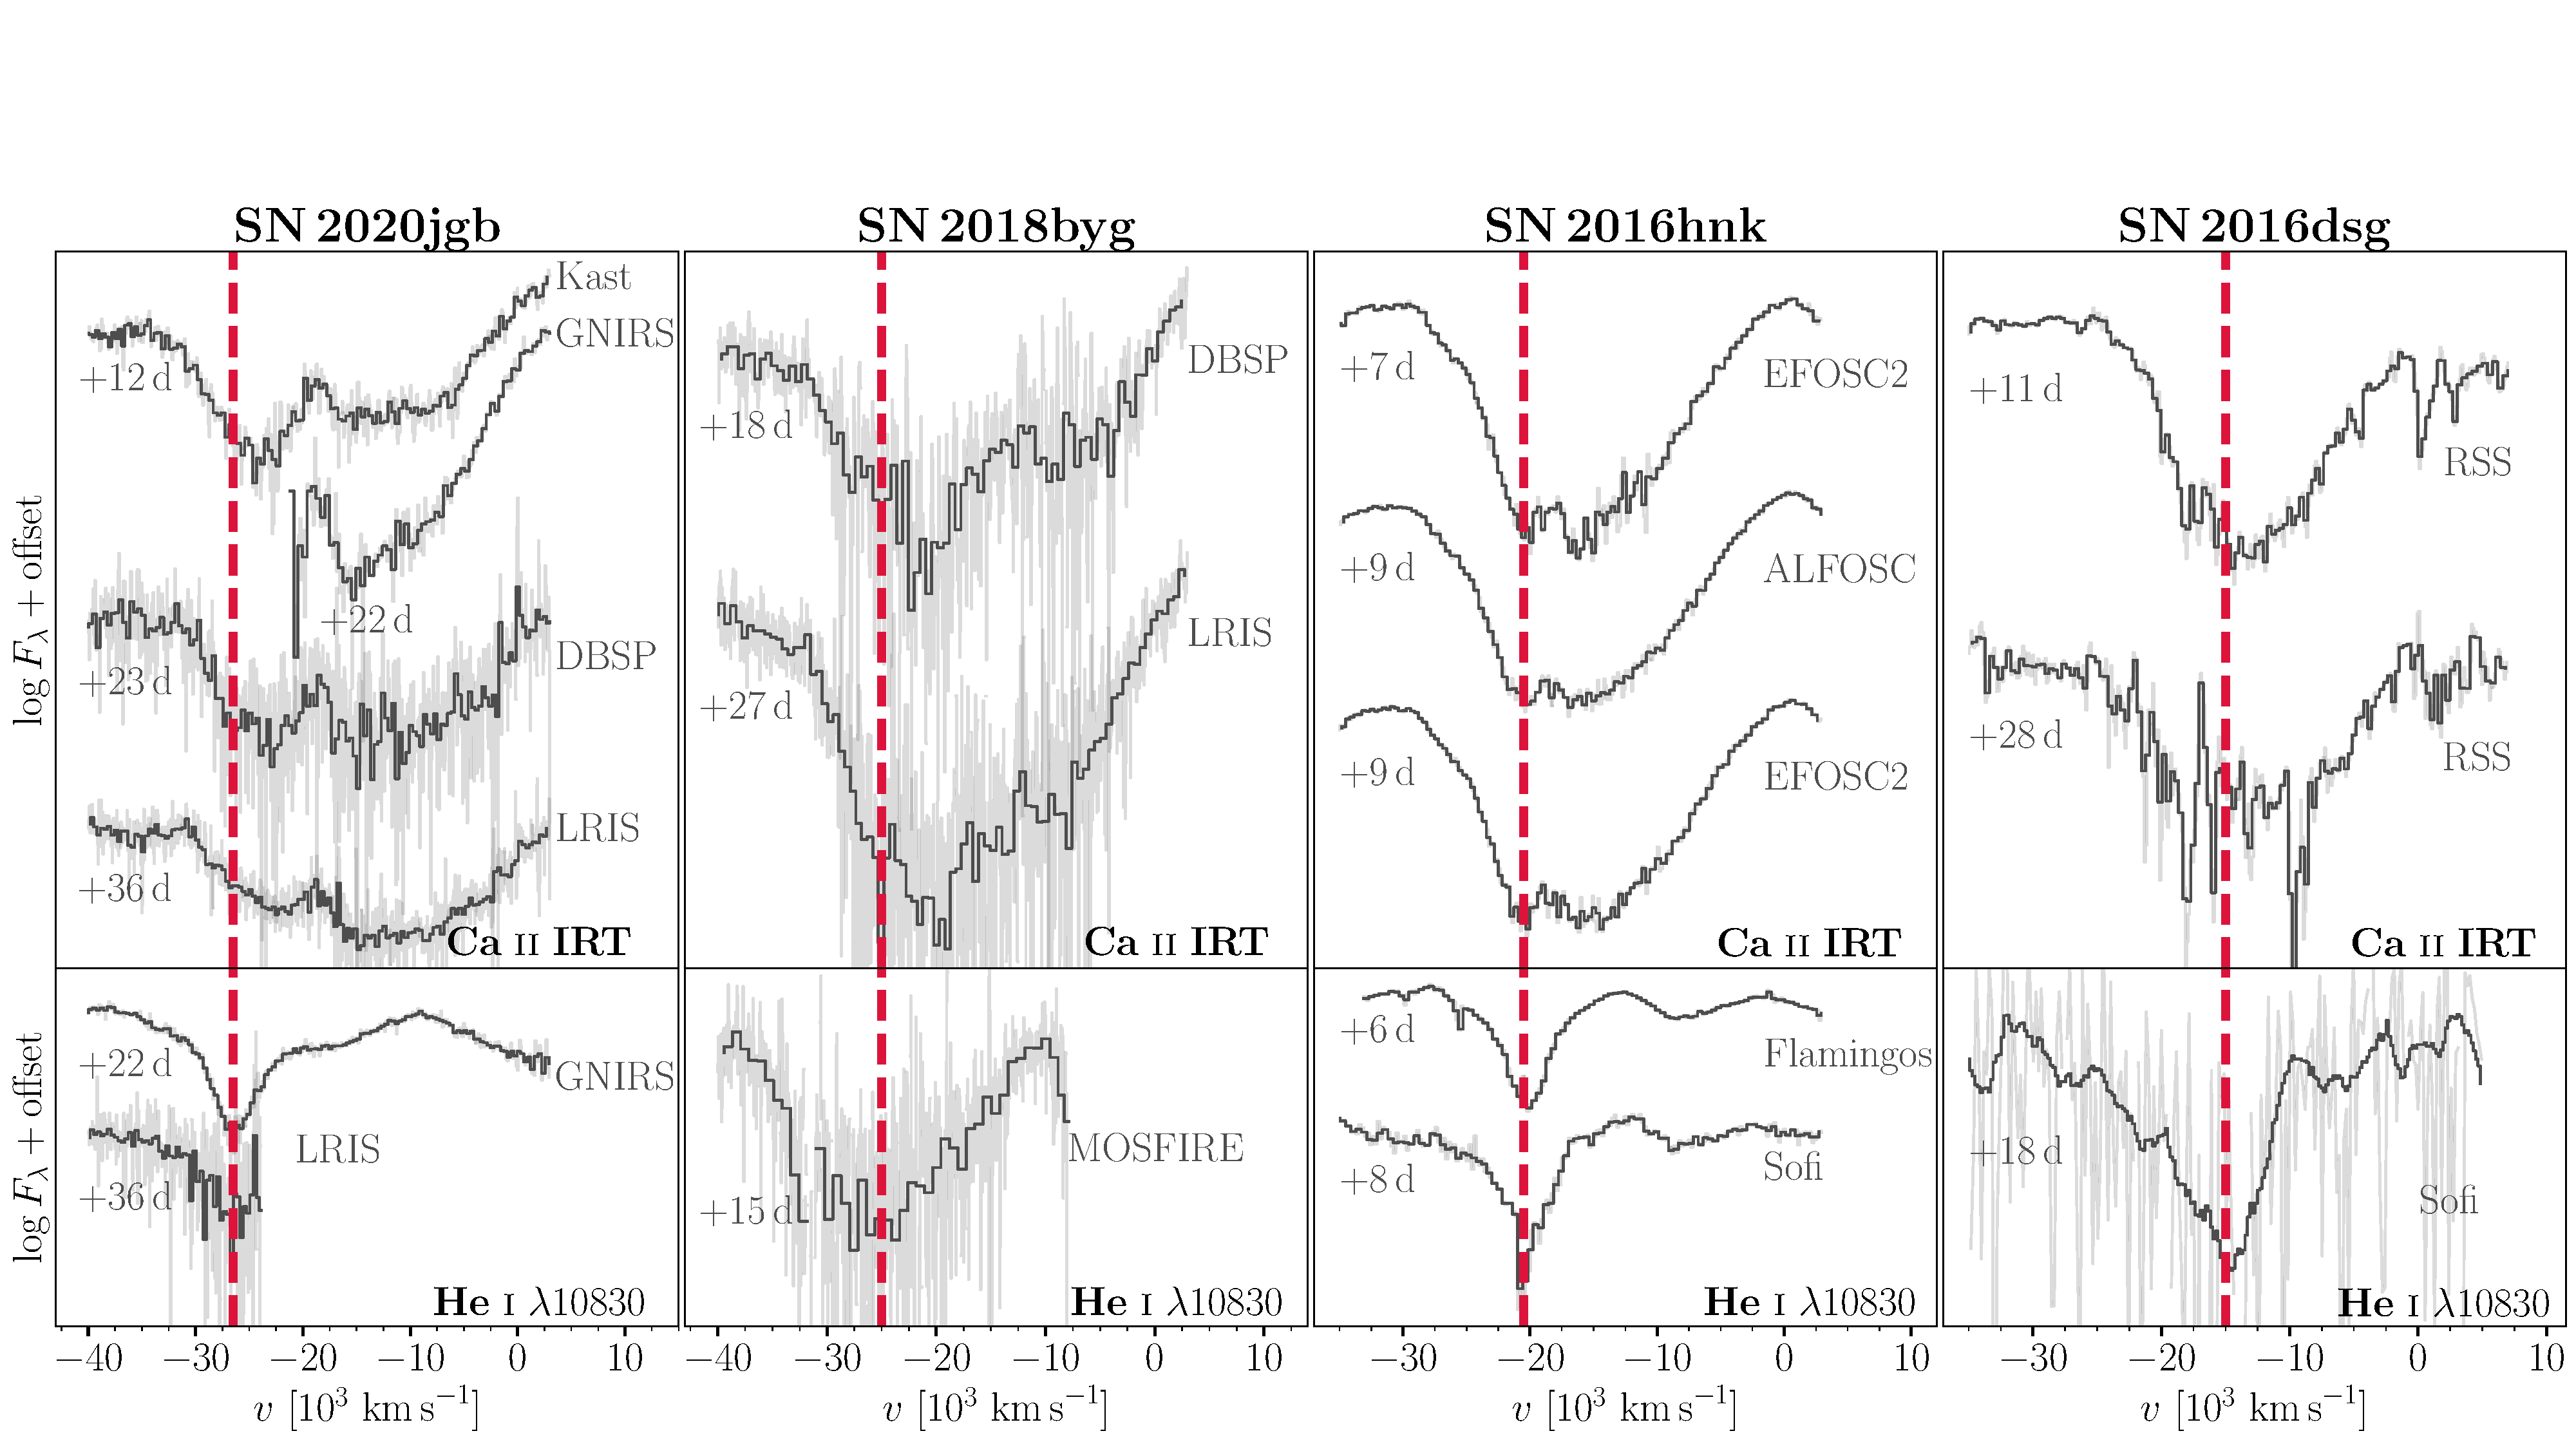
\includegraphics[width=\linewidth]{CaII_HeI_hvf.pdf}
    \caption{Spectra in the velocity space, comparing the high-velocity component of \ion{Ca}{2} IRT and the absorption feature at $\approx$0.99 \micron\ assuming it is associated with \ion{He}{1} at 1.0830 \micron.}
    \label{fig:hvf_comp}
\end{figure}

Still, this helium detection remains skeptical, since other \ion{He}{1} are not unambiguously detected, such as the \ion{He}{1} $\lambda$2.0581 \micron. Considering a line velocity of $\approx$26,000 km/s and a host galaxy redshift of 0.0307, this line will be blueshifted to $\approx$1.95 \micron\ in the observer frame, so will be strongly blended by the strong telluric lines within 1.8-2.0 \micron. After telluric correction, the signal to noise ratio reaches $\sim$5, with which we still cannot see any significant absorption feature. An upper limit of the equivalent width is determined to be $<2\%$ of the 1.0830 \micron\ line, while theoretically, the 2.0581 \micron\ line is supposed to be only a factor of 6-12 weaker, depending on temperature \citep{Marion2009_NIR}. Another fact is that the 1 \micron\ feature is as strong as the \ion{He}{1} $\lambda$1.0830 \micron\ in many helium-rich core-collapse supernovae, say, Type Ib supernovae, in which the \ion{He}{1} $\lambda$2.0581 \micron\ is weaker than the 1.0830 \micron line yet still prominent \citep{CSP_Ibc_2022}. If the 1 \micron feature is associated with \ion{He}{1}, it would be very unusual if the 2 \micron\ feature is not seen at all, even if somehow blended by the telluric lines. 

Other possibilities include the \ion{Mg}{2} $\lambda$1.0927 \micron, the \ion{C}{1} $\lambda$1.0693 \micron, and the \ion{Fe}{2} $\lambda$1.0500 \micron\ \& $\lambda$1.0863 \micron. The \ion{Mg}{2} $\lambda$1.0927 \micron\ is prevalent in the NIR spectra of SNe Ia, but usually disappears within a week after the peak luminosity \citep{Marion2009_NIR}, while our spectra were obtained three weeks/a month after the peak. A stronger \ion{Mg}{2} line at 0.9227 \micron\ is not detected either. Also, the problematically high radial velocity of $\approx$30,000 km/s is not seen in normal SNe Ia, and is over 20\% faster than the HVF of \ion{Ca}{2} IRT at the same phase.

The \ion{C}{1} $\lambda$1.0693 \micron\ line from the unburnt carbon is much less frequently seen than the \ion{Mg}{2} $\lambda$1.0927 \micron. \citet{hsiao_CSP_2019} presented a sample of five SNe Ia with \ion{C}{1} detections, showing the \ion{C}{1} feature is strongest for those fainter, fast-declining objects. However, in their sample, the \ion{C}{1} feature is always accompanied by the stronger \ion{Mg}{2} 1.0927\micron\ line, and is a pre-maximum feature which fades away as the luminosity peaks. The required expansion velocity for \ion{C}{1} is $\approx$22,000 km/s, which is consistent with the HVF of \ion{Ca}{2} IRT, but still overwhelmingly faster than the estimated velocity for the sample in \citet{hsiao_CSP_2019} ($\sim$10,000-12,000 km/s).

The \ion{Fe}{2} features in SNe Ia usually start to develop three weeks after the peak, about the same phase when we got our GNIRS spectrum. Two \ion{Fe}{2} lines, $\lambda$0.9998 \micron\ and $\lambda$1.0500, are actually visible on each of the wing of the 1 \micron\ feature. The \ion{Fe}{2} $\lambda$1.0863 \micron\ line is not yet seen. They correspond to an expansion velocity of $\approx$8,000 km/s, which is consistent with the PVF of the \ion{Ca}{2} IRT at the same epoch, and most matches the same two lines for normal SNe Ia \citep{Marion2009_NIR}, making the identification more reliable. Obviously, these two \ion{Fe}{2} features are wider and shallower than the strong feature between them. We fit the whole feature with three Gaussian profiles, two of which are set to be the blueshifted \ion{Fe}{2} $\lambda$0.9998 \micron\ and $\lambda$1.0500. We find that the shallower and wider \ion{Fe}{2} lines contributes to only $\sim$40\% of the total equivalent width, and the rest $\sim$60\% comes from the central feature, which cannot be accounted for by any \ion{Fe}{2} feature at the same velocity. Given the similarity of the Fe-group line blanketing between the GNIRS spectrum with the spectrum of SN 2004da at +25 days, the distribution of Fe-group elements inside each supernova ejecta should be somehow similar, so the central region of the 1 \micron\ feature is not likely to be associated with \ion{Fe}{2}.

\section{Host Galaxy} \label{sec:host}
\begin{figure}
    \centering
    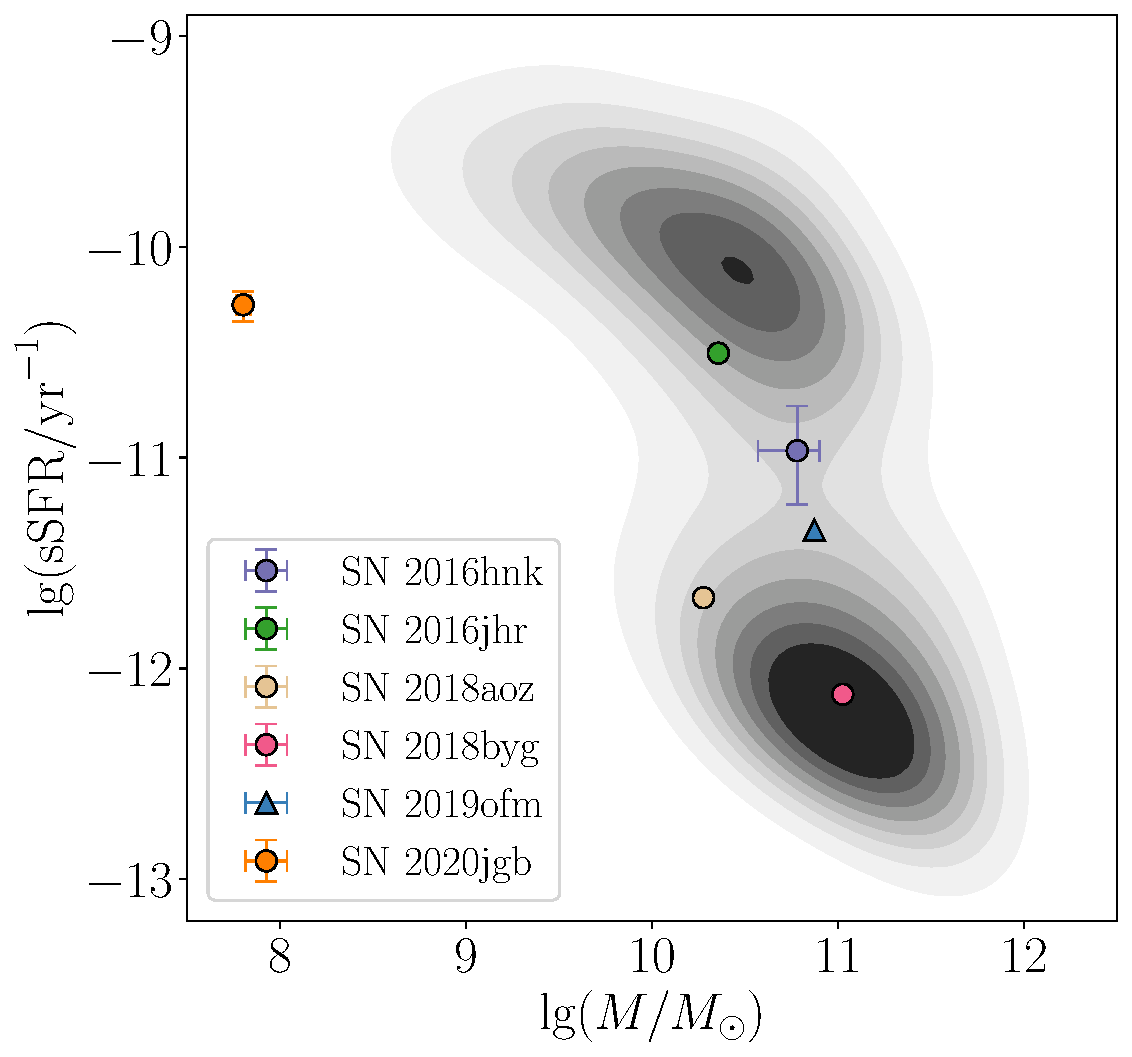
\includegraphics[width=\linewidth]{host.pdf}
    \label{fig:host}
    \caption{The specific star formation rate (sSFR) and the galactic mass for the host galaxies of He-shell double detonation candidates.}
\end{figure}

\section{Model Comparisons} \label{sec:model}

\section{Discussion and Conclusion} \label{sec:discussion}

\bibliography{SN2020jgb}{}
\bibliographystyle{aasjournal}

%% This command is needed to show the entire author+affiliation list when
%% the collaboration and author truncation commands are used.  It has to
%% go at the end of the manuscript.
%\allauthors

%% Include this line if you are using the \added, \replaced, \deleted
%% commands to see a summary list of all changes at the end of the article.
%\listofchanges

\end{document}

% End of file `sample631.tex'.
